\chapter{Previsione I parziale}
\subsubsection{Quando}
Settimana 17-23 aprile.

\subsubsection{Argomenti}
\begin{description}
    \item[E-R:] abbiamo un testo in linguaggio naturale, dobbiamo creare uno schema concettuale con il linguaggio di modellazione E-R.
    \item[M-R:] abbiamo un piccolo testo, dobbiamo trovarne le chiavi primarie, i vincoli di integrità, i vincoli di dominio. 
\end{description}
Di solito è più facile il secondo esercizio, ma è importante fare bene il primo per poi fare il secondo.

\section{Modello dei dati relazionale}
Relazione -> teoria degli insiemi -> tramite sql
\\Due modelli:
\begin{itemize}
    \item modello a documenti (no-sql)
    \\si usa come strumento mongodb
    \item modello a serie temporali (time series)
\end{itemize}

\chapter{DBMS}
\section{Linguaggi per basi di dati}
Diversi tipi:
\begin{description}
    \item[L. per definizione dei dati:] Data Definition Languages - DDL
    \\ Si occupano della definizione degli schemi logici, fisici e delle autorizzazioni di accesso.
    \item[L. di manipolazione dei dati:] Data Manipulation Languages - DML
    \\Si occupano dell'interrogazione (\textbf{consultazione}) e aggiornamento (\textbf{manipolazione}) delle basi di dati.
\end{description}
Alcuni linguaggi come SQL (Structured Query Language) hanno funzioni di entrambe le categorie.

\subsection{Pagine web statiche/dinamiche}
Codice sorgente: linguaggio di \textit{scripting} (che usa dei \textit{tag}) HTML che è un linguaggio statico, che non permette dinamicità dei contenuti. Deve essere interpretato.
\\Sono nati altri linguaggi (tipo \textbf{php}, asp, jsp, etc...) che sono più \textit{dinamici} e riescono a replicare meglio le richieste dell'utente generando contenuti on-demand.
\\Quando una pagina dinamica deve mostrare i dati, accede ad una base di dati volta per volta per recuperare informazioni da mostrare.
\\Viene fatta una \textbf{query} per \textbf{accedere} ad una sezione ben definita di dati (es. informazioni di un utente sul sito Esse3 delle segreterie).
\\Posso fare una query anche per \textbf{manipolare} i dati (es. iscrizione ad un esame).

\section{Personaggi ed interpreti}
\begin{itemize}
    \item \textbf{progettisti} e realizzatori di \textbf{DBMS};
    \item \textbf{progettisti della base di dati} e amministratori della base di dati (DBA);
    \\Questi dovrebbero avere pieni poteri senza sforare nella "privatezza" dei dati.
    \\Def. dalle slides: Persona o gruppo di persone responsabile del controllo centralizzato e della gestione del sistema, delle prestazioni, dell'affidabilità, delle autorizzazioni. 
    \\Le funzioni del DBA includono quelle di progettazione, anche se in progetti complessi ci possono essere distinzioni.
    \item \textbf{progettisti} e programmatori \textbf{di applicazioni};
    \item \textbf{utenti}:
    \\- utenti finali (terminalisti): eseguono applicazioni predefinite (transazioni)
    \\- utenti casuali: eseguono operazioni non previste a priori, usando linguaggi interattivi
\end{itemize}

\section{Un esercizio per ripassare quanto detto}
\subsection{Es1}
Quali delle seguenti affermazioni sono vere?
\begin{itemize}
    \item l'indipendenza dei dati permette di scrivere programmi senza conoscere le strutture fisiche dei dati
    \\\textbf{VERO}
    \item l'indipendenza dei dati permette di modificare le strutture fisiche dei dati senza dover modificare i programmi che accedono alla base di dati
    \\\textbf{VERO}
    \item l'indipendenza dei dati permette di formulare interrogazioni senza conoscere le strutture fisiche
    \\\textbf{VERO}
\end{itemize}

\subsection{Es2}
Quali delle seguenti affermazioni sono vere?
\begin{itemize}
    \item il fatto che le basi di dati siano condivise
    permette di ridurre ridondanze e inconsistenze
    \item il fatto che le basi di dati siano persistenti ne
    garantisce l'affidabilità
    \\\textbf{VERO}
    \item il fatto che le basi di dati siano condivise rende
    necessaria la gestione della privatezza e delle
    autorizzazioni
    \\\textbf{VERO}
\end{itemize}

\subsection{Es3}
Quali delle seguenti affermazioni sono vere?
\begin{itemize}
    \item le istruzioni DML permettono di interrogare la base di dati ma non di modificarla
    \\\textbf{VERO}
    \item le istruzioni DDL permettono di specificare la struttura della base di dati ma non di modificarla
    \item 
    – non esistono linguaggi che includono sia istruzioni
    DDL sia istruzioni DML
    – SQL include istruzioni DML e DDL
    – le istruzioni DML permettono di interrogare la base
    di dati e di modificarla
    \\\textbf{VERO}
\end{itemize}

da sistemare
\\Gli esercizi che seguono sono utili per fissare i concetti, ma non ai fini dell'esercizio dell'esame.
\\
\\Cambia il pacco di slides.

\chapter{Progettazione di una base di dati}
Atzeni, Ceri, Paraboschi, Torlone, capitoli 6 e 7.
\\In questa parte del corso studieremo come
progettare una base di dati...
\\Verra’ illustrato ed esemplificato il processo di
progettazione concettuale e logica delle basi di dati
relazionali, che permette, partendo dai requisiti di
utente, di arrivare a produrre strutture di basi di dati di
buona qualità.
\\La progettazione di basi di dati è una delle attività
del processo di sviluppo dei sistemi informativi va
quindi inquadrata in un contesto più generale: il ciclo
di vita dei sistemi informativi

\section{Metodologie e modelli}
Un concetto importante di un'applicazione è \textbf{il ciclo di vita}.
\\\textbf{Def.:} insieme e sequenzializzazione delle attività svolte da analisti, progettisti, utenti, nello sviluppo e nell’uso dei sistemi informativi.
\\Attività iterativa, quindi “un ciclo”.
\begin{center}
    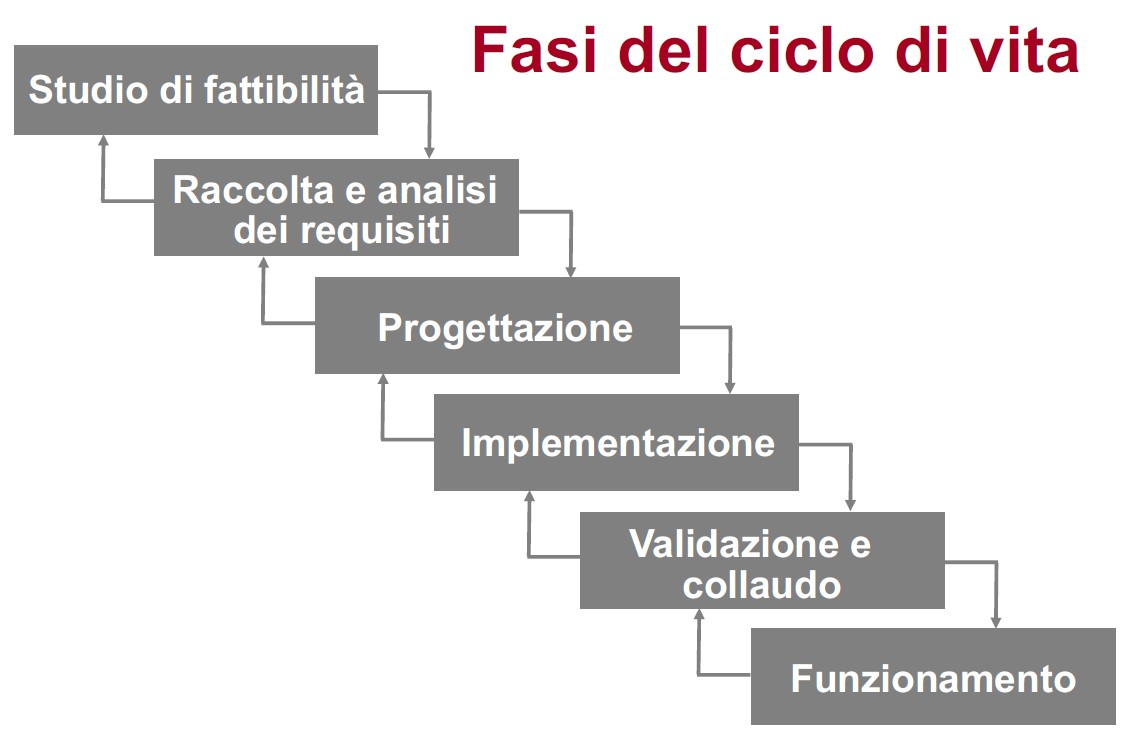
\includegraphics[width=0.75\textwidth]{chaptersLezioniSara/img/ciclo_di_vita1.jpg}
\end{center}
\begin{description}
    \item[Studio di fattibilità:] il progettista ha a che fare col committente (cliente) 
    \item[Raccolta e analisi dei requisiti:] viene prodotto un documento con i requisiti
    \item[Progettazione:] ER -> PL (?)
    \item[Implementazione:] si comincia
    \item[Validazione e collaudo:] di volta in volta, ci si confronta con l'utente o si controlla almeno di star seguendo i requisiti
    \item[Funzionamento:] non ho capito ma credo sia la fase finale, quindi la consegna del progetto finito. GUARDA LA SLIDE 8
\end{description}
Noi ci concentreremo sulla parte di progettazione, in particolare sulla modellizzazione dei dati.
\begin{center}
    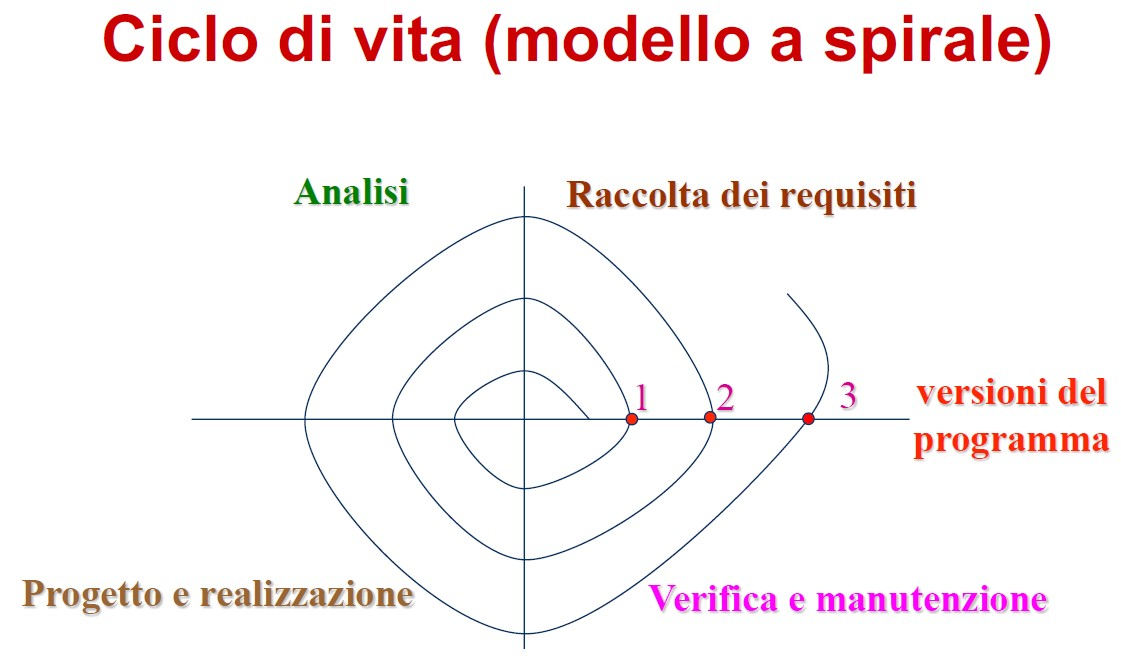
\includegraphics[width=0.75\textwidth]{chaptersLezioniSara/img/ciclo_di_vita2.jpg}
\end{center}
Ha balzato le slide di progettazione ma guardale.

\section{Progettazione}
Tre fasi:
\begin{center}
    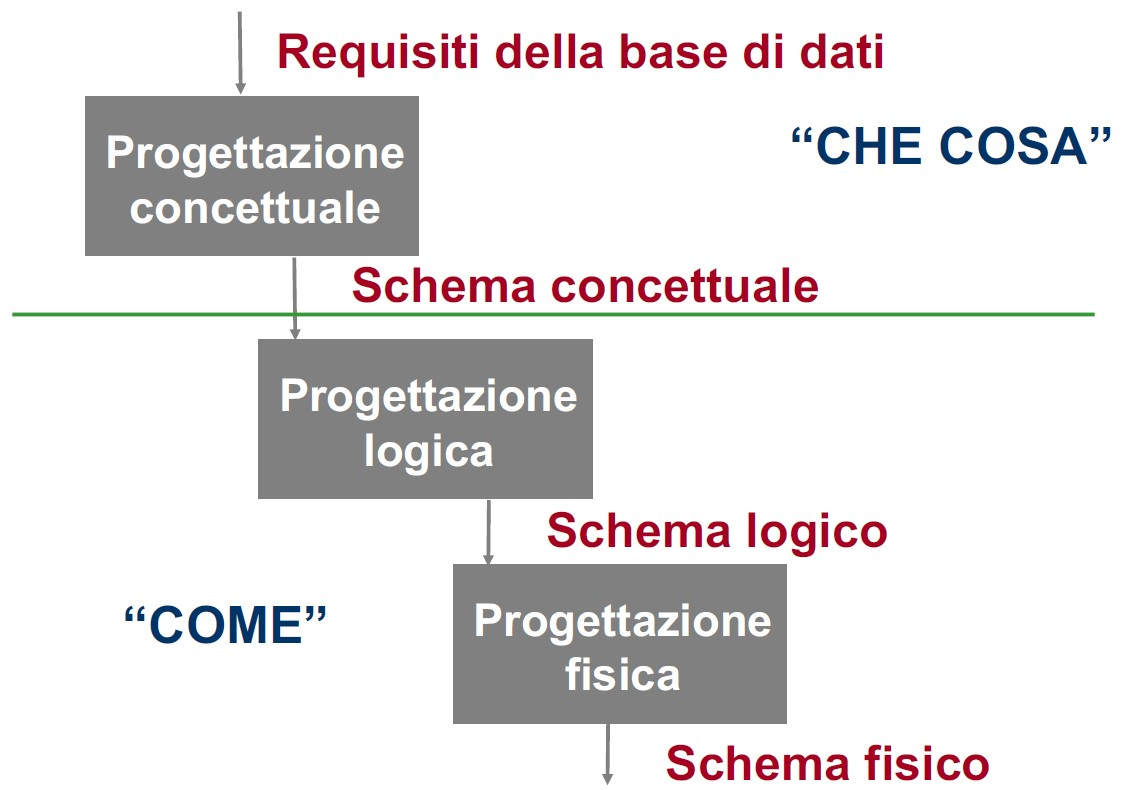
\includegraphics[width=0.75\textwidth]{chaptersLezioniSara/img/progettazione2.jpg}
\end{center}
A lezione vedremo p. concettuale e p. logica. La p. fisica sarà affrontata a laboratorio.
\begin{center}
    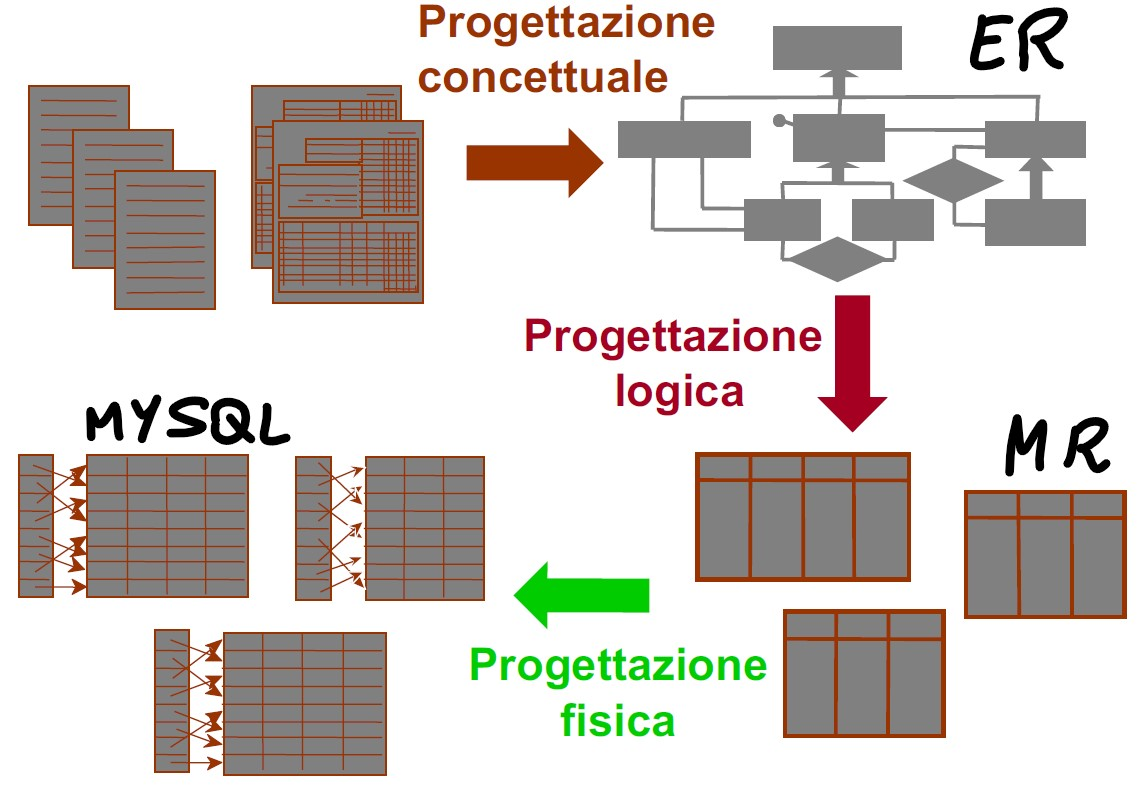
\includegraphics[width=0.75\textwidth]{chaptersLezioniSara/img/progettazione3.jpg}
\end{center}

\subsection{Fase di progettazione concettuale}
Progettazione concettuale: traduce i requisiti del sistema
informatico in una descrizione formalizzata, integrata delle
esigenze aziendali, espressa in modo indipendente dalle scelte
implementative (DBMS, SW e HW).
formale: la descrizione deve essere espressa con un
linguaggio non ambiguo e capace di descrivere in modo
soddisfacente il sistema analizzato;
integrata: la descrizione deve essere in grado di descrivere
nella globalità l'ambiente analizzato;
indipendente dall'ambiente tecnologico: la descrizione deve
concentrarsi sui dati e sulle loro relazioni, e non sulle scelte
implementative.

\subsection{Fase di progettazione logica}
La progettazione logica consiste nella traduzione dello
schema con concettuale nel modello dei dati del DBMS
Il risultato è uno schema logico, espresso nel DDL
del DBMS
In questa fase si considerano anche aspetti legati ai vincoli
ed all'efficienza
La progettazione logica si articola in due sotto-fasi:
•ristrutturazione dello schema concettuale
•traduzione verso il modello logico

\subsection{Fase di progettazione fisica}
Progettazione concettuale: traduce i
requisiti el sistema informatico in una descrizione
formale, integrata e indipendente dalle scelte
implementative (DBMS, SW e HW).
Progettazione logica: traduce lo schema
concettuale nel modello di rappresentazione
dei dati adattato dal DBMS scelto
Progettazione fisica: completa lo schema
logico ottenuto con le specifiche proprie
dell'hw/sw scelto. Il risultato e' lo schema
fisico che descrive le strutture di
memorizzazione ed accesso ai dati

\chapter{Introduzione al modello Entità-Relazione}
\section{Modello Entità-Relazione}
\begin{center}
    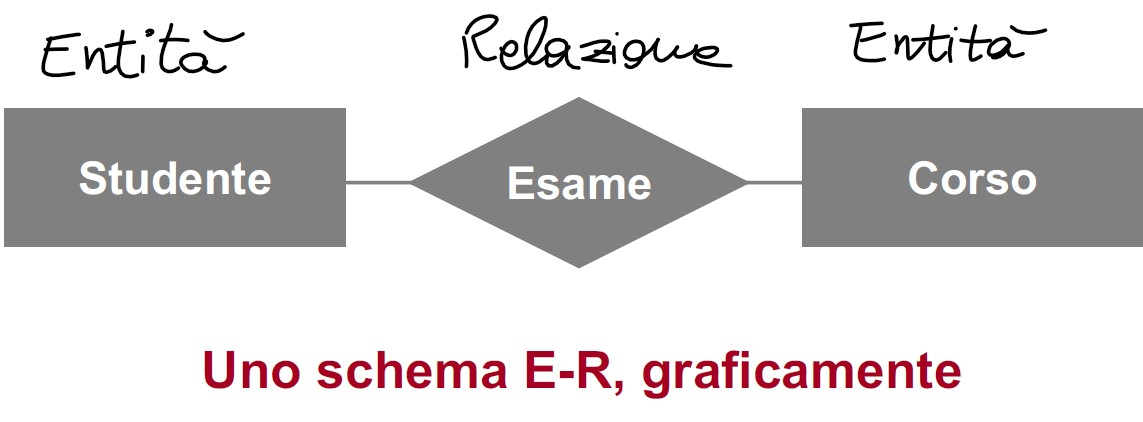
\includegraphics[width=0.75\textwidth]{chaptersLezioniSara/img/ER1.jpg}
\end{center}
Il modello ENTITÀ-RELAZIONE (E-R) è un
linguaggio grafico semi-formale per la
rappresentazione di schemi concettuali
•Il modello E-R si è ormai affermato come uno
standard nelle metodologie di progetto e nei sistemi
SW di ausilio alla progettazione
•Ne esistono molte versioni, (più o meno) diverse
l'una dall'altra.
•Entity-Relationship, P.P. Chen 1976

\`E una sottosezione di UML

\section{Entità}
\textbf{Def.:} Classe di oggetti (fatti, persone, cose) della applicazione di interesse con proprietà comuni e con esistenza “\textbf{autonoma}” e della quale si vogliono registrare fatti specifici.
\\\textit{Esempi:}
\begin{itemize}
    \item impiegato
    \item dipartimento
    \item città
    \item conto corrente
    \item università
    \item studente
\end{itemize}
L'essere autonoma di un'entità è un concetto fondamentale: es. gli studenti sono entità, gli esami sostenuti no perché non hanno un'esistenza autonoma.
\\\`E importante imparare, mentre stiamo leggendo un testo in linguaggio naturale, a capire chi può essere un'entità.
\subsection{Formalismi}
Si rappresentano con un rettangolo:
\begin{center}
    \includegraphics[width=0.75\textwidth]{chaptersLezioniSara/img/Entità1.jpg}
\end{center}
Ogni entità ha un nome che la identifica univocamente nello schema:
\begin{itemize}
    \item nomi espressivi
    \item opportune convenzioni (singolare)
\end{itemize}
A livello estensionale un'entità è costituita da un insieme di oggetti, che sono chiamati le sue istanze.
\\Ciò significa che, se in uno schema $S$ è definita una entità $E$, in ogni istanza $I$ dello schema $S$, alla entità $E$ è associato un insieme di oggetti (che viene denotato $istanze(I,\, E)) {e1, e2, e3, ..., e_n}$ (si chiama parte estensionale) che viene detto anche l'estensione di $E$ nella istanza $I$ dello schema $S$.
\\Una istanza di entità non è un valore che identifica un oggetto, ma è l'oggetto stesso.

\subsection{Occorrenza (o istanza) di entità}
\begin{itemize}
    \item 
•oggetto della classe che l'entità rappresenta
•Nello schema concettuale rappresentiamo le
entità, non le singole istanze (“astrazione”)
Quindi:
CONOSCENZA ASTRATTA -> entità
CONOSCENZA CONCRETA ->istanza di entità
\end{itemize}

\section{Attributi}
Un attributo di entità è una proprietà locale di un'entità,
di interesse ai fini dell'applicazione
• Un attributo associa ad ogni istanza di entità un valore
appartenente ad un insieme detto dominio dell'attributo
(tipicamente, interi, caratteri, stringhe, ecc.)
• Si definisce un attributo per l'entità E quando si vuole
rappresentare una proprietà locale delle istanze
dell'entità E.
Una proprietà di un oggetto si dice locale quando in
ogni istanza dello schema il valore di tale proprietà
dipende solamente dall'oggetto stesso, e non ha alcun
rapporto con altri elementi dell'istanza dello schema

\begin{center}
    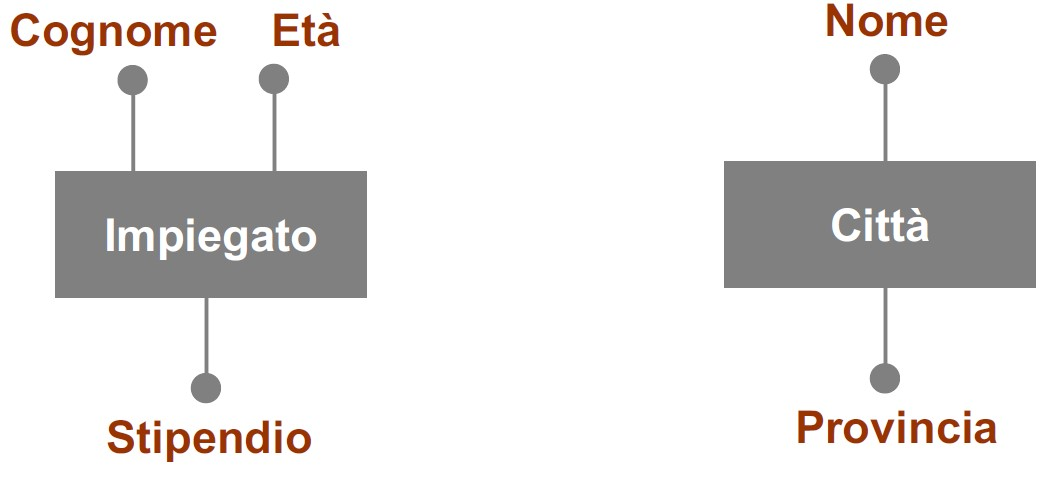
\includegraphics[width=0.75\textwidth]{chaptersLezioniSara/img/Attributi1.jpg}
\end{center}
Ogni attributo di entità ha un nome che lo identifica in modo
univoco nell'ambito della entità, ed è rappresentato da un
cerchio collegato alla entità a cui appartiene.

\begin{center}
    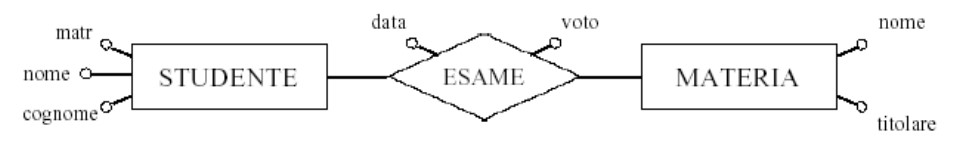
\includegraphics[width=0.75\textwidth]{chaptersLezioniSara/img/Attributi2.jpg}
\end{center}
Ogni attributo e' definito su un dominio di valori.
Un attributo associa ad ogni istanza di entità o associazione
un valore nel corrispondente dominio.
I domini solitamente non vengono specificati nell'E-R ma nella
documentazione associata. Se li si vuole indicare, la
notazione e' la seguente
\begin{center}
    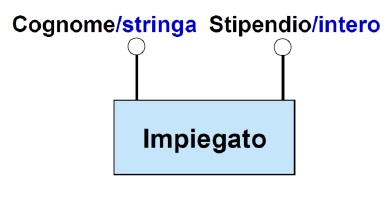
\includegraphics[width=0.75\textwidth]{chaptersLezioniSara/img/Attributi3.jpg}
\end{center}
Una entità può avere o no attributi.

\subsubsection{Attributi di entità}
\begin{center}
    \includegraphics[width=0.75\textwidth]{chaptersLezioniSara/img/Attributi_entità1.jpg}
\end{center}
Un'entità non può avere più di un valore per attributo. E non può averne neanche meno (oddio, veramente cambia in base al contesto, se ci fossero attributi facoltativi avrei dei \textbf{nulli}).
\\Gli attributi hanno un dominio, che ci specifica di che tipo di dati stiamo parlando.
\subsubsection{Attributi nulli}
I \textit{nulli} sono un concetto fondamentale nelle basi di dati.
\subsubsection{Attributi composti}
Si ottengono raggruppando attributi di una medesima entità o relazione che presentano affinità nel loro significato o uso.
\begin{center}
    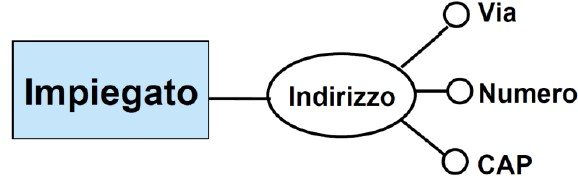
\includegraphics[width=0.75\textwidth]{chaptersLezioniSara/img/Attributi_composti.jpg}
\end{center}

\section{Relazione - Associazione}
Fatto che descrive un'azione o una situazione e che stabilisce legami logici tra istanze di entità (associa, mette in relazione) nella realtà che stiamo considerando.
\\I legami possono essere fra piu' di due entita'. Il numero di entità coinvolte in una relazione determina il suo grado (si vedano prossime slide).
\\NB: spesso useremo il termine ASSOCIAZIONE o RELATIONSHIP (per relazione) evitando confusione con la terminologia relazionale.
\subsection{Formalismi}
Si rappresentano con un rombo:
\begin{center}
    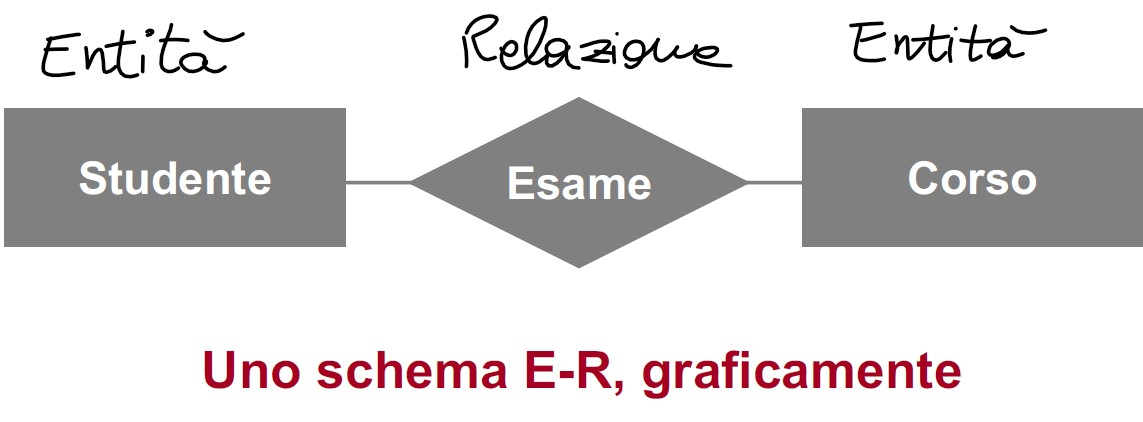
\includegraphics[width=0.75\textwidth]{chaptersLezioniSara/img/ER1.jpg}
\end{center}
Ogni relazione ha un nome che la identifica univocamente nello schema:
\begin{itemize}
    \item nomi espressivi
    \item opportune convenzioni (singolare, sostantivi invece che verbi)
\end{itemize}
A livello estensionale una relazione R tra le entità E ed F è
costituita da un insieme di coppie (x,y), tali che x è una istanza
di E, ed y è una istanza di F. Ogni coppia è detta istanza della
relazione R
• Ciò significa che, se in uno schema S è definita una relazione
R sulle entità E ed F, in ogni istanza I dello schema S, alla
relazione R è associato un insieme di coppie (denotato da
istanze(I,R)) {(x1, y1), (x2, y2), (x3, y3), …}
che viene detto anche l’estensione di R nella istanza I dello
schema S
• In altre parole, una relazione nel modello ER è, dal punto di
vista della semantica, una relazione matematica. In ogni
istanza I dello schema S si ha:
\begin{center}
    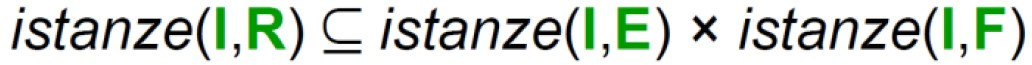
\includegraphics[width=0.75\textwidth]{chaptersLezioniSara/img/Relazioni1.jpg}
\end{center}

\subsection{Istanze di associazione}
\textbf{Def.:} combinazione (aggregazione) di istanze di entità che prendono parte alla associazione.
\\Es.:
•Rossi insegna Basi di dati
•Batini appartiene all’Università di Milano Bicocca
•La ditta Rossi ordina PC
•Bianchi lavora al magazzino 4
•Il tornio K22 è installato nell’officina 37
•il TIR 542 viaggia sulla tratta NA-MI

Es.:
\\Dalla semantica delle relazioni segue immediatamente che non possono esistere due istanze della stessa relazione che coinvolgono le stesse istanze di entità.
\begin{center}
    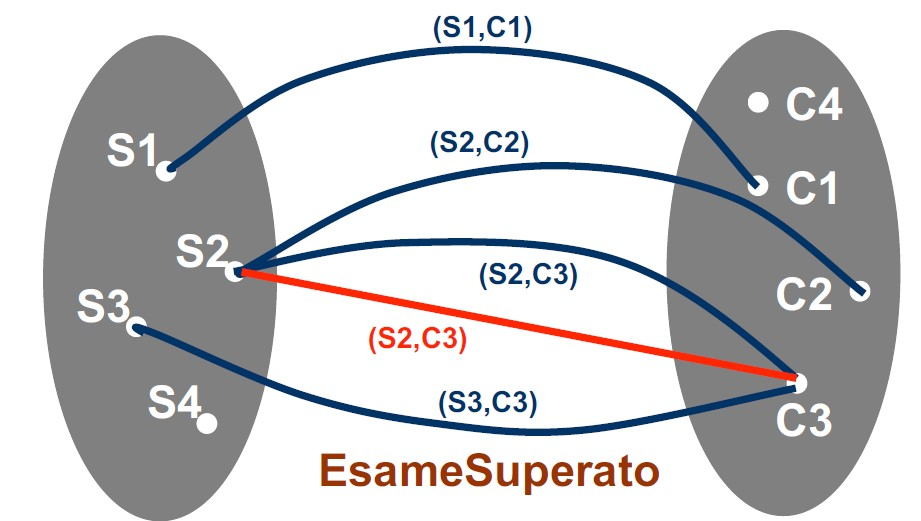
\includegraphics[width=0.75\textwidth]{chaptersLezioniSara/img/Relazioni2.jpg}
\end{center}
N.B.: due entità possono essere coinvolte in più relationship.
\begin{center}
    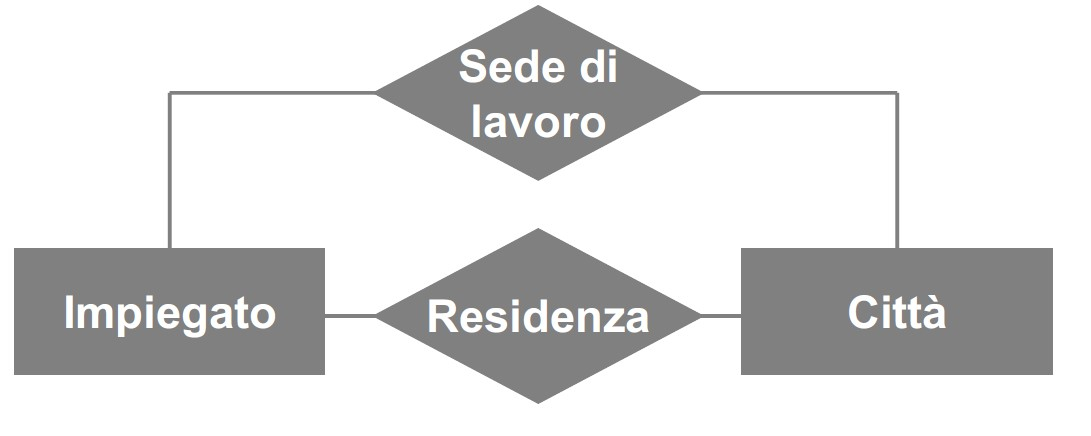
\includegraphics[width=0.75\textwidth]{chaptersLezioniSara/img/Relazioni3.jpg}
\end{center}
Le relationship possono coinvolgere più di due entità.
\begin{center}
    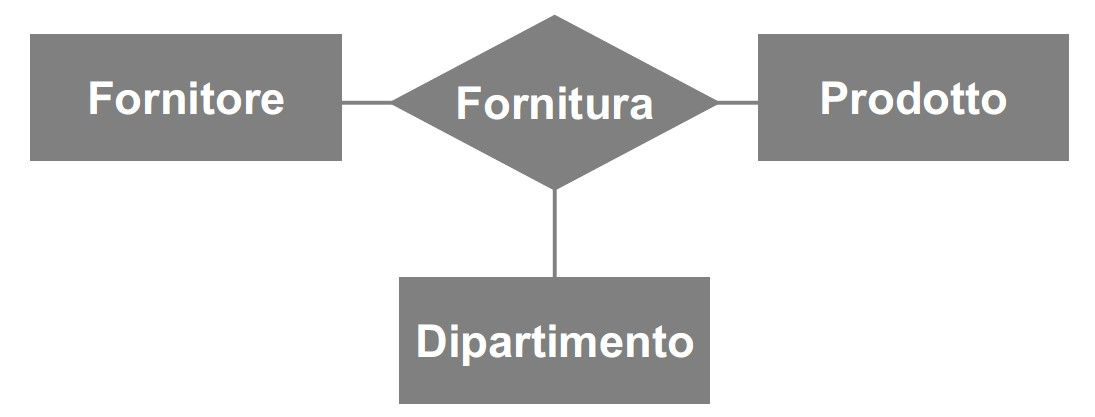
\includegraphics[width=0.75\textwidth]{chaptersLezioniSara/img/Relazioni4.jpg}
\end{center}

\subsubsection{Relazioni n-arie}
\begin{center}
    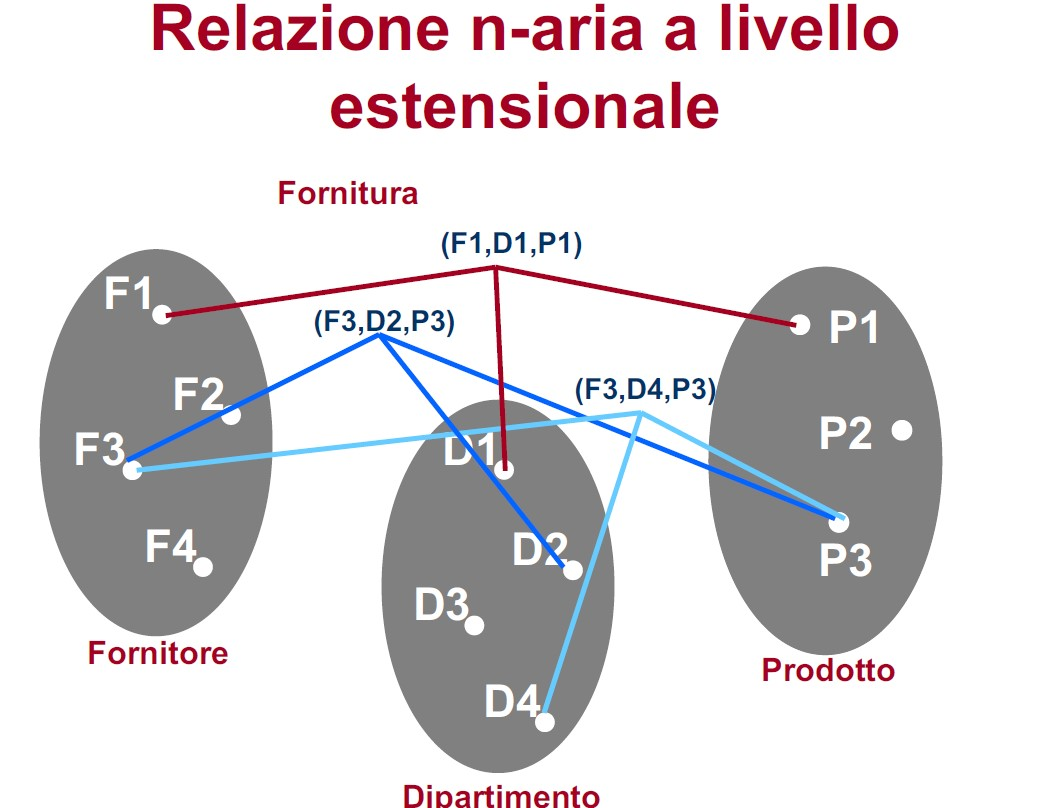
\includegraphics[width=0.75\textwidth]{chaptersLezioniSara/img/Relazioni5.jpg}
\end{center}
A livello estensionale (ovvero in ogni istanza I dello
schema S) una relazione R tra le entità E1,E2,…,En è
costituita da un insieme di n-ple (o tuple) (x1,x2,…,xn),
tali che x1 è una istanza di E1 in I, x2 è una istanza di
E2 in I,…, xn è una istanza di En in I. Ogni n-pla è detta
istanza della relazione R nella istanza I dello schema S
• Quindi, in ogni istanza I dello schema si ha:
\begin{center}
    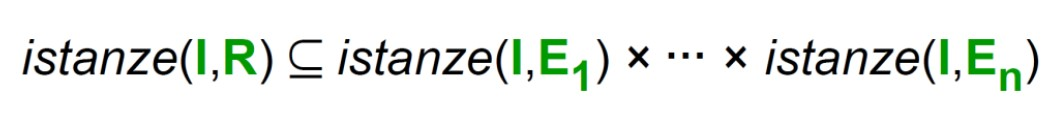
\includegraphics[width=0.75\textwidth]{chaptersLezioniSara/img/Relazioni6.jpg}
\end{center}

Una relazione può avere o no attributi.

\subsubsection{Attributi di relazione}
Un attributo di relazione è una proprietà locale di una
relazione, di interesse ai fini dell’applicazione
• Un attributo della relazione R tra le entita E1,E2,…,En
modella una proprietà non di E1, non di E2,…, non di
En, ma del legame tra E1,E2,…,En rappresentato da
R
• Un attributo associa ad ogni istanza di relazione un
valore appartenente ad un insieme detto dominio
dell’attributo

\subsubsection{Formalismi}
Ogni attributo di relazione ha un nome che lo identifica in
modo univoco nell’ambito della relazione, ed è
rappresentato da un cerchio collegato alla relazione a cui
appartiene.
\begin{center}
    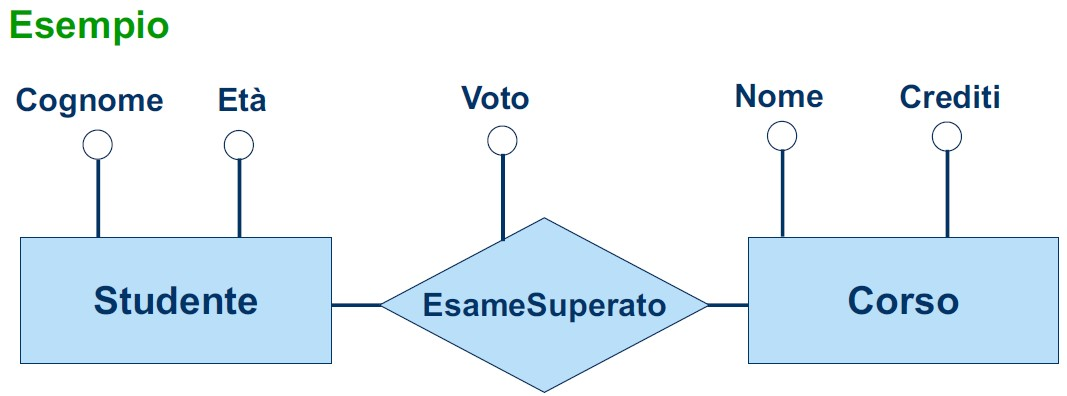
\includegraphics[width=0.75\textwidth]{chaptersLezioniSara/img/Attributi_relazione1.jpg}
\end{center}

Ho perso un po' di slides

\section{Entity-Relationship}


BLOB: Binary Long OBject. Sono i pallini pieni della rappresentazione degli attributi di entità.

cose

Es.
Descrivere lo schema concettuale della seguente realtà:
I docenti hanno un codice fiscale ed una età. I docenti operano nei corsi di laurea
(si dice che afferiscono ai corsi di laurea). Interessa la data di afferenza dei docenti
ai corsi di laurea. I corsi di laurea hanno un codice ed un nome, ed appartengono
alle facoltà. Ogni facoltà ha un nome.
\begin{center}
    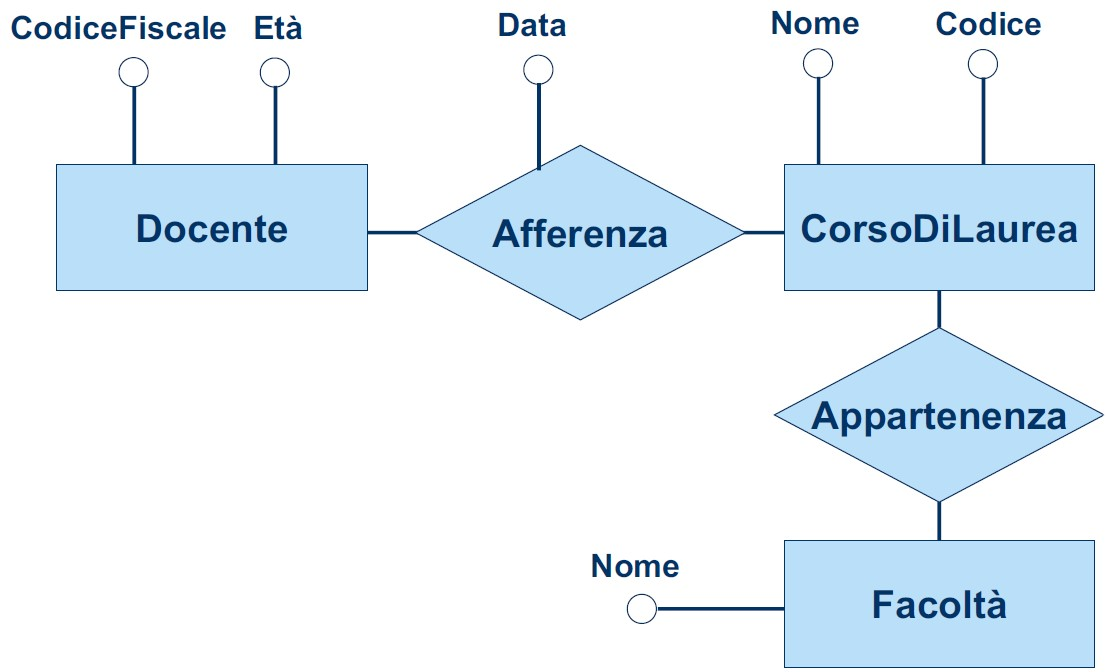
\includegraphics[width=0.75\textwidth]{chaptersLezioniSara/img/ER_es1_sol.jpg}
\end{center}

\subsection{Relazioni ricorsive}
Una associazione può coinvolgere “due o più volte” la stessa entità (associazione ricorsiva o ad anello). Questo ovviamente la fa classificare come relazione \textbf{binaria}, anche se c'è rappresentata una sola entità noi stiamo facendo una relazione tra due istanze di quell'entità, quindi conta come due.
\begin{center}
    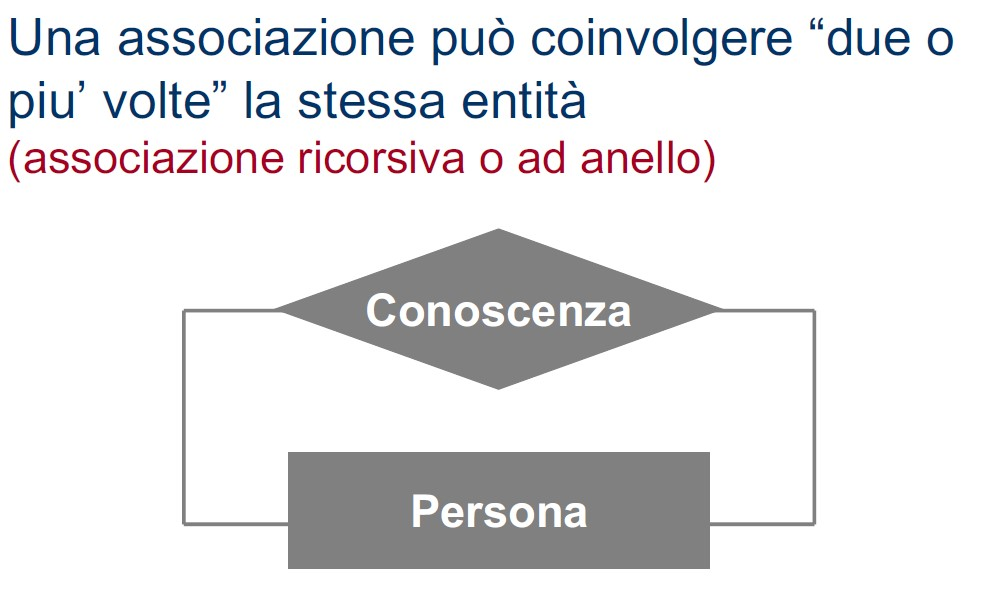
\includegraphics[width=0.75\textwidth]{chaptersLezioniSara/img/Relazioni_ricorsive1.jpg}
\end{center}
Ma siamo in grado da questo grafico di capire "chi viene prima e chi viene dopo"? No, se non operiamo sulla relazione: questo lo si fa aggiungendo dei "\textbf{ruoli}" alla relazione.
\begin{center}
    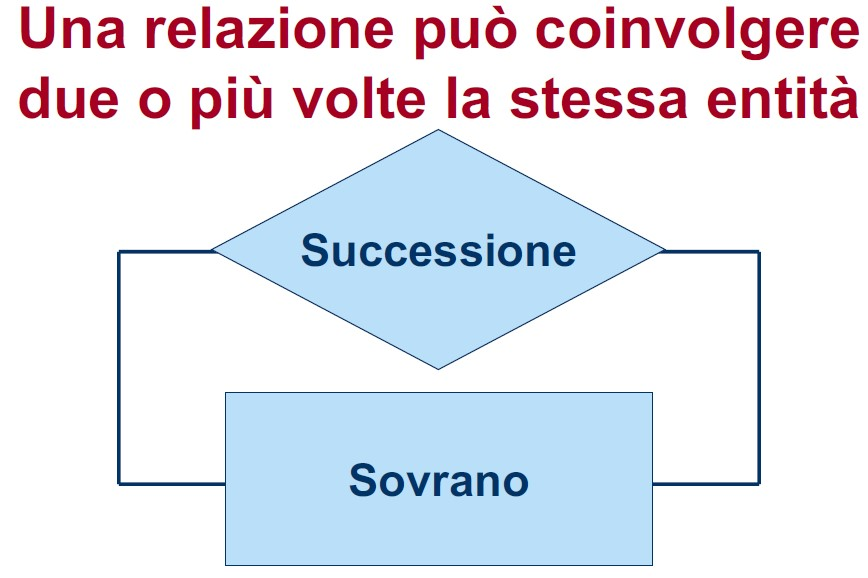
\includegraphics[width=0.75\textwidth]{chaptersLezioniSara/img/Relazioni_ricorsive2.jpg}
\end{center}
Problema: in una istanza di questo schema, data una coppia che è istanza di “Successione”, non si può individuare chi è il sovrano predecessore e chi il sovrano successore.
\subsubsection{I ruoli}
Nelle relazioni dove una stessa entità è coinvolta più volte è necessario aggiungere la specifica dei “ruoli”.

\subsubsection{Proprietà delle rel. ricorsive}
Un'associazione ad anello può essere o meno:
\begin{itemize}
    \item Simmetrica: $(a,\, b) \in A \Rightarrow (b,\, a) \in A$
    \item Riflessiva:$(a,\, a) \in A$
    \item Transitiva:$(a,\, b) \in A,  (b,\, c) \in A \Rightarrow (a,\, c) \in A$
    \item L'associazione conoscenza è simmetrica, irriflessiva e intransitiva.
\end{itemize}


vabbeh mancano slides

ultima cosa vista: esempio dei docenti uno migliore dell'altro